\documentclass{beamer}
% Class options include: notes, handout, trans
%                        

\usepackage[french]{babel}
\usepackage[utf8]{inputenc}
\usepackage{tikz}

% Theme for beamer presentation.
\usepackage{beamerthemesplit} 
% Other themes include: beamerthemebars, beamerthemelined,beamerthemetree, beamerthemeplain

\usefonttheme{professionalfonts}

\title[Création d'un interface graphique pour Tikz]{Création d'un interface graphique pour Tikz}
\subtitle{PSTL encadré par Fréderic Pechanski}    % Enter your title between curly braces
%\author[L. Numbers]{Lucas Numbers}                 % Enter your name between curly braces
\author[]{Ancelin Maxime\\Diakhate Aminata}                 % Enter your name between curly braces
\institute[UPMC]{M1 Informatique spécialité STL\\UPMC}      % Enter your institute name between curly braces
\date{8 juin 2012}      % Enter the date or \today between curly braces

\usepackage{graphicx}

\begin{document}

\newenvironment{violetpar}{\color{violet}}{}
\newenvironment{bluepar}{\par\color{blue}}{\par}
\newenvironment{yellowpar}{\par\color{orange}}{\par}




%\renewcommand{\labelitemi}{$\bullet$}

%%%%%%%%%%%%%%%%%%%%%%%%===Slide 1 - Titre
\begin{frame}
  \titlepage
\end{frame}

%%%%%%%%%%%%%%%%%%%%%%%%===Slide 2 - Plan
\begin{frame}
\frametitle{Plan} 

\begin{itemize}

\item Objectifs du PSTL

\item Réalisation du projet

\item Résultats

\item L'avenir de TikzG

%\item Predefined colors are          % COLORS!!!!
%        \textcolor{blue}{blue}, \textcolor{red}{red}, \textcolor{black}{black},
%        \colorbox{blue}{\textcolor{white}{white}},
 %       \textcolor{cyan}{cyan}, \textcolor{magenta}{magenta},
  %      \textcolor{yellow}{yellow}, \textcolor{green}{green}.
%
 %       Define colors?  Colored formulae?  You bet!
  %        \verb2\definecolor{darkgreen}{rgb}{0,0.4,0}2
   %             \definecolor{darkgreen}{rgb}{0,0.4,0}
    %    \\ \textcolor{darkgreen}{$A = \pi r^2$}:


\end{itemize}
\end{frame}

%%%%%%%%%%%%%%%%%%%%%%%%===Slide 3 - OBJECTIFS DU PSTL
\begin{frame}
\frametitle{Objectifs du PSTL} 


\begin{itemize}

\item Création d'une interface graphique pour
faciliter\\ l'utilisation de Tikz.

\item Sous-ensemble de Tikz traité : nœuds,
arêtes.

\end{itemize}
\end{frame}

%%%%%%%%%%%%%%%%%%%%%%%%===Slide 4 - Réalisation du projet
\begin{frame}
\frametitle{Réalisation du projet} 


\begin{itemize}

\pause \item Transformation du code Tikz en image

\pause \item Création de l'interface graphique

\pause \item Représentation mémoire des objets Tikz

\pause \item Intéraction avec le graphe

\end{itemize}

\end{frame}

\begin{frame}
\frametitle{Transformation d'un code Tikz en image}
\centering
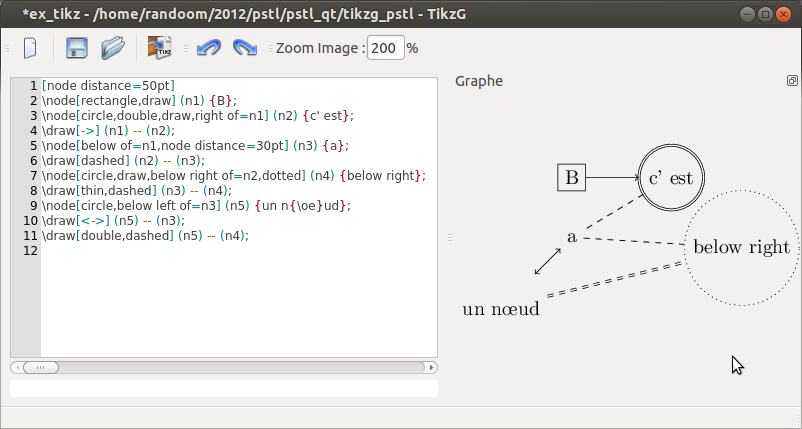
\includegraphics[width=10cm, height=6cm]{img/r_1.png}
\end{frame}


\begin{frame}
\frametitle{Transformation d'un code Tikz en image}
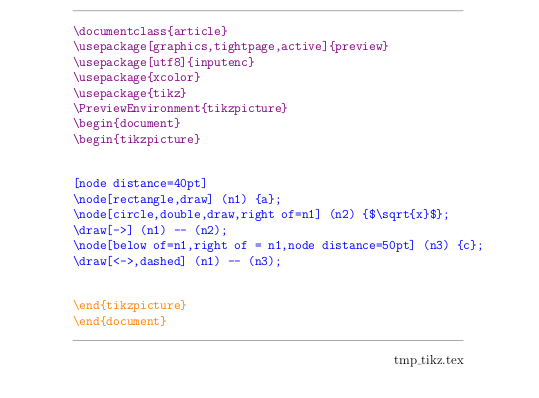
\includegraphics[width=10cm, height=4cm]{img/c1.png} \\
\begin{center}
$\overset{pdflatex -halt-on-error tmp_tikz.tex > /dev/null}{\downarrow}$

\includegraphics[width=5cm, height=0.5cm]{img/re1.png} \\
$\overset{convert}{\downarrow}$ \\

\includegraphics[width=5cm, height=0.5cm]{img/re2.png} \\
\end{center}

\end{frame}

\begin{frame}

\frametitle{Représentation mémoire des objets Tikz}

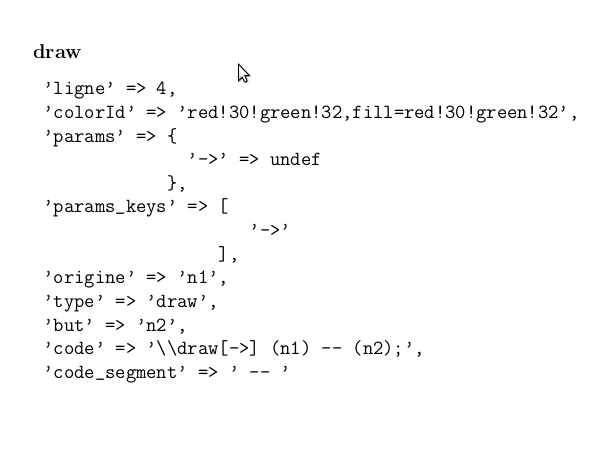
\includegraphics[width=5cm, height=5cm]{img/n3.png}
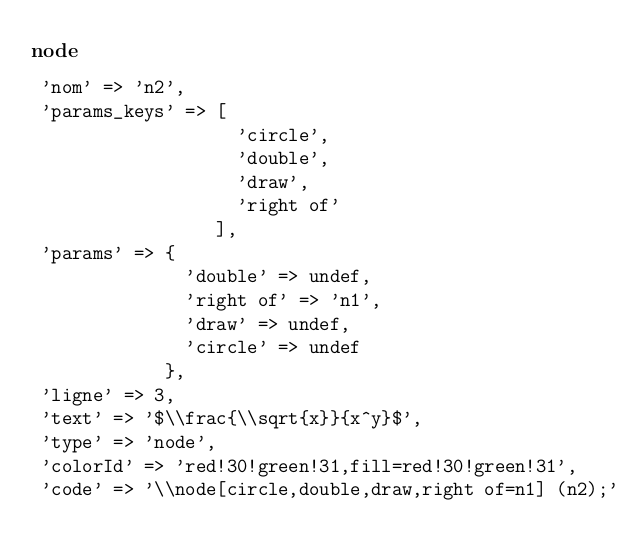
\includegraphics[width=7cm, height=5cm]{img/n2.png}\\
\centering
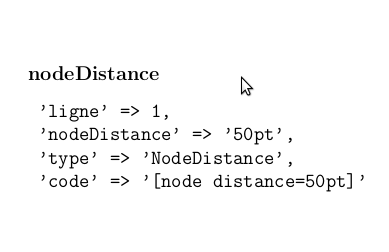
\includegraphics[width=5cm, height=3cm]{img/n1.png}
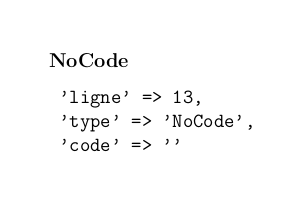
\includegraphics[width=5cm, height=3cm]{img/n4.png}
\end{frame}

\end{document}
